%==========================================================================
\chapter{Conceptual Interfaces for Inputting Problem Data}
\label{Conceptual Interfaces}

\section{What are conceptual interfaces?}

In Figure \ref{fig-conceptual-interface} we present an illustration
of the philosophy behind conceptual interfaces.

%[Cut and paste from Rob's paper. Now it needs editing].

\begin{figure}
\centering
\includegraphics[width=5in]{concep_iface.eps}
\caption{%
Graphic illustrating the notion of conceptual interfaces.
All of these elements are not necessarily in \hypre{}.}
\label{fig-conceptual-interface}
\end{figure}

The top row of Figure \ref{fig-conceptual-interface} 
illustrates a number of conceptual interfaces.  Generally,
the conceptual interfaces are denoted by different types of computational
grids,  but other application features might also be used, such as
geometrical information.  
These conceptual interfaces are intended to represent the
way that applications developers naturally think of their linear problem, and
provide natural interfaces for them to pass the data that defines
their linear system into \hypre{}. 
Essentially, these conceptual interfaces can be considered  
convenient utilities for helping a user build a matrix data structure
for \hypre{} solvers and preconditioners.
For
example, applications that use structured grids (such as in the left-most
interface in the Figure ~\ref{fig-conceptual-interface})
typically view their linear problems in terms of
stencils and grids.  On the other hand, applications that use unstructured
grids and finite elements typically view their linear problems in terms of
elements and element stiffness matrices.  Finally, the right-most interface is
the standard linear-algebraic (matrix rows/columns) way of viewing the
linear problem.

The second row of Figure ~\ref{fig-conceptual-interface} is a set of linear solver algorithms.
Each linear solver group requires different information from the user through
the conceptual interfaces.  So, the geometric multigrid algorithm (GMG) listed
in the left-most box, for example, can only be used with the left-most conceptual
interface.  On the other hand, the ILU algorithm in the right-most box may be
used with any conceptual interface. 

The third row of Figure ~\ref{fig-conceptual-interface} is a list of data layouts or matrix/vector storage
schemes.  The relationship between linear solver and storage scheme is similar
to that of interface and linear solver.


\section{Which conceptual interface should I use?}

\hypre{} currently supports three conceptual interfaces:

\begin{itemize}

\item
\code{Finite Element Interface:}
This is appropriate for users who form their linear systems from
a finite element discretization.
The interface mirrors typical finite element data structures,
including element stiffness matrices.
Though this interface is provided in \hypre{}, its definition
was determined elsewhere (www.z.ca.sandia.gov/fei).

\item
\code{Structured Grid Interface:}
This interface is appropriate for applications whose grids
consist of unions of logically rectangular grids with a fixed
stencil pattern of nonzeros at each grid point.
Contributions to the matrix are made in terms of the stencils.
{\bf NOTE:} The current version only supports a single unknown
per grid point, though an extended interface that includes
multiple unknowns is under construction.

\item
\code{IJ interface:}
This is the traditional linear algebraic interface. 
It can be used as a last resort by users for whom the other
grid-based interfaces are not appropriate.
It requires more work on the user's part, though still less than
building parallel sparse data structures.
General solvers and preconditioners are available through this
interface, but not specialized solvers which need more information.
Our experience is that users with legacy codes, in which they already
have code for building matrices in particular formats, find the
IJ interface relatively easy to use.

\end{itemize}

Generally, a user should choose the most specific interface
that matches their application, because this will allow them
to use more specialized and more efficient solvers and preconditioners
without losing access to more general solvers.